\section{Thermostat Design}
\label{proposal}
We propose to explore and develop an end-to-end Linux Prototype supported with
minimal hardware changes to employ slower but cheaper memory technologies in
data-centers providing higher capacity at lower cost of ownership.

\subsection{Identifying HotSpots in Cold Hugepages}

%\begin{figure}[t]
%\centering
%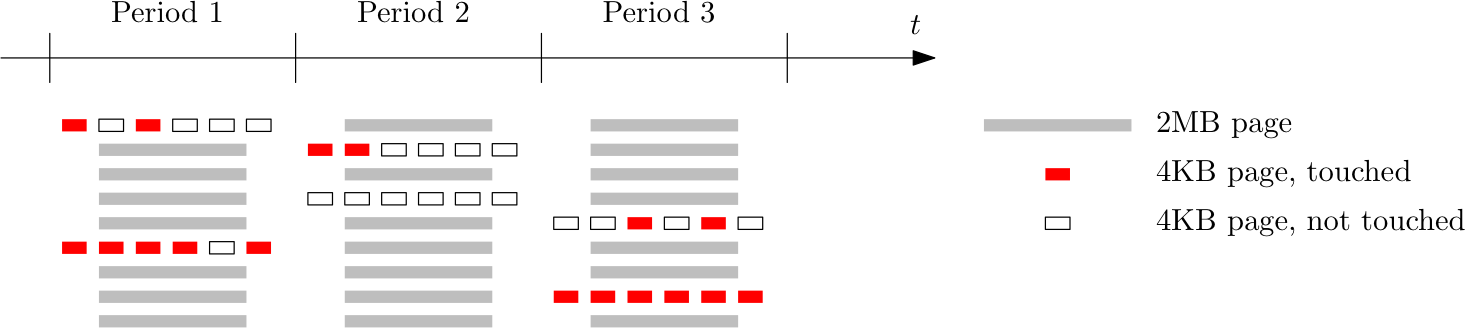
\includegraphics[width=1.0\columnwidth]{thermostat/figures/sampling.png}
%\caption{Sampling to identify HotSpot pages in otherwise cold page}
%\vspace{-0.175in}
%\label{fig:sampling}
%\end{figure}
To solve this situation, we propose to build a dynamic controller (which we call
Thermostat) that can decide when to {\it break} a huge page into several regular
pages, and place some of those smaller pages which are deemed to be cold in
slower but cheaper memory. We will implement Thermostat as a part of custom
Linux prototype.

The Thermostat controller has to distinguish between ``hotSpot'' hot pages --
ones with only a few hot data blocks, and ``uniform'' hot pages -- ones where a
significant fraction of the data blocks in that page are hot.  We propose to
build such a classification mechanism that is at once a)
application-transparent, i.e., no source code change in the application should
be necessary, b) low-overhead, so as to not degrade the performance benefits of
using THP, and, c) high-accuracy, i.e., most of the classified ``hotSpot'' pages
are indeed hotspots (low false positives) and most of the pages classified
``uniform'' are {\it} not in fact hotspots (low false negatives).

We observe that there are hot 4KB pages present within 2MB huge pages.
Figure~\ref{fig:motivation-thermostat} shows that applications on average have
$\approx$ 50\% of cold data. As we change page size form 4KB to 2MB fraction of
cold data reduced by $\approx$ 20\%. Page granularity based OS mechanisms cannot
reveal the hot portions within huge pages. Hence, we propose a sampling based
page temperature measurement mechanism that classifies pages by their access
rate.

%
%\begin{figure}[t]
%\centering
%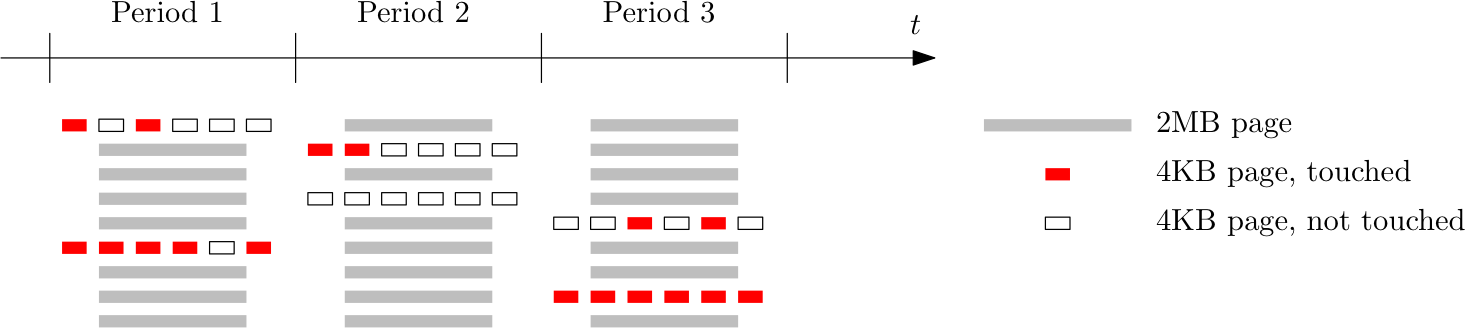
\includegraphics[width=1.0\columnwidth]{thermostat/figures/sampling.png}
%\caption{TLB and PTE changes}
%\vspace{-0.175in}
%\label{fig:motivation}
%\end{figure}
%
%\subsection{Sampling Mechanism}
%The Thermostat controller needs an effective mechanism for chunking up a DRAM
%huge page into several small pages, and also for compacting several small hot
%pages into a single DRAM huge page. Chunking up a huge page is relatively simple
%-- one need only allocate several page table entries (PTEs) corresponding to the
%chunked up page. Doing the inverse, that is compacting several small pages from
%the slow-mem and DRAM into a single DRAM huge page has more challenges. First,
%due to memory fragmentation, it may not be possible to find a suitable space to
%put the newly created huge page. Second, reading several small pages from
%slow-mem, and creating a huge page out of them can be a potentially very long
%latency operation, which can then affect application throughput as well as tail
%latency. We plan to study the design trade-off space of when to perform
%these operations and incorporate the obtained insights into building the Thermostat
%controller.
\subsection{Translation Facades}
Thermostat will divide application pages into categories: (1) Extremely hot huge
pages -- pages with high access rates, (2) Extremely cold huge pages -- pages
with low access rates, and (3) ``hotSpot'' huge pages -- cold 2MB page with
certain 4KB hot regions. We will put extremely hot huge pages in fast memory and
extremely cold huge pages in slow memory. However, there are following
challenges in placing {\it hotSpot} huge pages in either of the fast memory or
slow memory technology: (1) placing them in slow memory can hurt performance due
to high access rates to 4KB hots spots in otherwise cold 2MB page, and (2)
placing them in DRAM will lead to in-efficient utilization of slow and cheaper
memory capacity.
%Another option is to break such {\it hotSpot} huge pages into
%regular pages and place hot 4KB pages in DRAM and cold 4KB pages in slow memory,
%but breaking such huge pages can potentially lead to loosing performance
%benefits of huge pages. In Redis we observe that there is a large fraction of
%{\it hotSpot} huge pages with more than 15\% of 4KB pages wihtin 2MB pages being
%hot. Hence, none of the above techniques can fully exploit the potential savings
%of placing large fraction of pages in cheaper slow memory, while still reaping
%the performance benefits of THP.
%
%Therefore, we propose ``translation facades'', a mechanism that remaps a portion
%of a 2MB mapping with alternate physical addresses or permissions at 4KB
%granularity. HotSpot pages will have multiple valid mappings, hot regions with
%valid 4KB mapping and cold regions with valid 2MB mapping. We propose to modify TLB
%and page table structures to support such multiple mappings.

As a solution to both these problems, we plan to experiment the following two
approaches. The first approach is to break such {\it hotSpot} huge pages into
regular pages and place hot 4KB pages in DRAM and cold 4KB pages in slow memory.
A significant upside of such an approach is that it can be implemented without
any significant hardware changes. However, breaking such huge pages can
potentially lead to losing performance benefits of huge pages. For example, in
Redis we observe that there is a large fraction of {\it hotSpot} huge pages ($>$
30\% of total pages).

As a second approach, we propose ``translation facades'', a mechanism that
remaps a portion of a 2MB mapping with alternate physical addresses at 4KB
granularity. HotSpot pages will have multiple valid mappings, hot regions with
valid 4KB mappings and cold regions with a single valid 2MB mapping. We propose
to modify TLB and page table structures to support such multiple mappings.
